

    \item Consider an elliptically shaped rail PQ in the vertical plane with OP \( = 3 \) m and OQ \( = 4 \) m. A block of mass 1 kg is pulled along the rail from P to Q with a force of 18 N, which is always parallel to line PQ (see the figure given). Assuming no frictional losses, the kinetic energy of the block when it reaches Q is \( (n \times 10) \) Joules. The value of \( n \) is \underline{\hspace{2.5 cm}}, (take acceleration due to gravity \( = 10 \, \text{m/s}^2 \))
    
    \begin{center}
        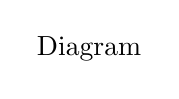
\begin{tikzpicture}
            \node {Diagram};
        \end{tikzpicture}
    \end{center}

